% Chapter Abstract
In this chapter, we construct a simple description of \gws as a consequence of \GR. In Section~\ref{1:sec:gravitational-radiation} we derive \gws as solutions of the Einstein field equations in a linearised gravity regime under the weak-field approximation. In Section~\ref{1:sec:gravitational-wave-detection} we will discuss the ground-based \gwadj observatories and how \gws will create physical effects that we can measure using these observatories. Finally, in Section~\ref{1:sec:modelling_CBC}, we model the gravitational waveform from the primary source of \gws---CBCs---we see with our detectors. For greater detail on any of these sections, readers are referred to the texts~\cite{Moore_book:2012, Schutz_book:2009, Maggiore_book:2007, Creighton_book:2009}.

\section{\label{1:sec:gravitational-radiation}Gravitational radiation}

Gravitational radiation refers to the propagation of perturbations in spacetime, predicted by \GR, that manifest as \gws. These waves are generated by the accelerated motion of massive objects and propagate at the speed of light. In this section, we will derive \gws as solutions to the Einstein field equations within the weak-field approximation, where the gravitational field is considered a small perturbation to flat spacetime. This approach, known as linearised gravity, allows for a simplified treatment of \gws and provides the foundation for understanding their key properties. We will also discuss the general characteristics of gravitational radiation, such as their polarisation and energy carried by \gws.

% Einstein field equations
Einstein's field equations (commonly referred to as Einstein's equations) are a set of $10$\footnote{Due to the symmetry of $G_{\mu\nu}$ and $T_{\mu\nu}$.} non-linear coupled equations which describe how the gravitational field is generated by matter and can be written eloquently using \GR notation as
%
\begin{eqnarray}
    G_{\mu\nu} = 8\pi T_{\mu\nu},
    \label{1:eqn:EFE}
\end{eqnarray}
%
where we use natural units, $G = c = 1$.

Einstein's equations relate the curvature of spacetime using the Einstein tensor, $G_{\mu\nu}$, to the stress-energy tensor, $T_{\mu\nu}$, which describes the density and flux of matter, energy, and momentum at each point in spacetime.

\subsection{\label{1:sec:perturbations}Perturbations in spacetime}

\Gws are a natural consequence of \GR and we show this by making a number of simplifications to Einstein's equations to reveal valid plane wave solutions. We begin in a flat-Minkowski spacetime, represented by the spacetime metric, $\eta_{\mu\nu}$, and make a \textit{weak} linear perturbation, $h_{\mu\nu}$ due to a gravitational field. In this scenario we can write the metric tensor, $g_{\mu\nu}$, as
%
\begin{equation}
    g_{\mu\nu} = \eta_{\mu\nu} + h_{\mu\nu},
    \label{1:eq:metric_perturbation}
\end{equation}
%
and to ensure our perturbation is small we enforce the condition $|h_{\mu\nu}| \ll 1$. In this regime, we are able to raise and lower indices using the Minkowski metric
%
\begin{equation}
    h^{\mu\nu} = \eta^{\mu\alpha}\eta^{\nu\beta}h_{\alpha\beta}.
    \label{1:eq:raise_lowering_indices}
\end{equation}
%
Terms of $h_{\mu\nu}$ greater than linear-order are negligible and are ignored, this is called taking the \textit{weak-field limit}. This simplification derives \gws in a regime where Einstein's equations are linearised, which significantly reduces the complexity of the calculations while still capturing the essential physical behaviour of \gws.

We can write the Einstein tensor, $G_{\mu\nu}$, in terms of the Riemann tensor, $R_{\mu\nu}$, the Ricci scalar, $R$, and the metric tensor
%
\begin{align}
    G_{\mu\nu} &= R_{\mu\nu} - \frac{1}{2}g_{\mu\nu}R,
    \label{1:eq:g_munu_riemann}
\end{align}
%
and we can introduce a quantity known as the \textit{trace reverse tensor}
%
\begin{equation}
    \Bar{h}_{\mu\nu} = h_{\mu\nu} - \frac{1}{2} \eta_{\mu\nu}h,
\end{equation}
%
where $h = \eta^{\mu\nu}h_{\mu\nu}$ is the trace of the metric perturbation.

We can then express the linearised Einstein tensor in terms of the linearised Riemann tensor and our trace reverse metric tensor~\cite{Moore_book:2012}
%
\begin{equation}
    R_{\mu\nu} - \frac{1}{2}g_{\mu\nu}R = \frac{1}{2}\left(\partial^{\sigma}\partial_{\mu}\Bar{h}_{\sigma\nu} - \partial^{\sigma}\partial_{\sigma}\Bar{h}_{\mu\nu} + \partial_{\nu}\partial^{\alpha}\Bar{h}_{\mu\alpha} - \eta_{\mu\nu}\partial^{\alpha}\partial^{\beta}\Bar{h}_{\alpha\beta}\right).
\end{equation}
%
We can then express our fully linearised Einstein field equations as
%
\begin{equation}
    - \Box\Bar{h}_{\mu\nu} + \partial^{\sigma}\partial_{\mu}\Bar{h}_{\sigma\nu}  + \partial_{\nu}\partial^{\alpha}\Bar{h}_{\mu\alpha} - \eta_{\mu\nu}\partial^{\alpha}\partial^{\beta}\Bar{h}_{\alpha\beta} = 16\pi T_{\mu\nu},
    \label{1:eq:linearised_efe}
\end{equation}
%
where $\Box$ is the flat space d'Alembertian operator,
%
\begin{equation}
    \Box = \partial^{\sigma}\partial_{\sigma} = -\frac{\partial^{2}}{dt^{2}} + \frac{\partial^{2}}{dx^{2}} + \frac{\partial^{2}}{dy^{2}} + \frac{\partial^{2}}{dz^{2}}.
\end{equation}
%

\subsection{\label{1:sec:gauge-transformations}Gauge transformations}

Inspecting Equation~\ref{1:eq:linearised_efe} we can identify the presence of the d'Alembertian operator $\Box$ along with terms involving divergences of $\bar{h}_{\mu\nu}$. Performing a gauge transformation to the 
harmonic gauge will eliminate the divergences,
%
\begin{equation}
    \partial^{\nu} \Bar{h}_{\mu\nu} = 0,
    \label{1:eq:divergence_gone}
\end{equation}
%
further simplifying our linearised Einstein equations.

In the weak-field limit we can make this gauge transformation by applying small coordinate translations to the perturbed spacetime that ensure the metric perturbations remain small,
%
\begin{align}
    x &\rightarrow x^{\prime}, \\
    x^{\prime\mu} &= x^{\mu} + \xi^{\mu}(x),
    \label{1:eq:gauge_transform}
\end{align}
%
where the metric in the new coordinate system is
%
\begin{equation}
    g^{\prime}_{\mu\nu} = \eta_{\mu\nu} + \bar{h}^{\prime}_{\mu\nu},
    \label{1:eq:gauge_metric}
\end{equation}
%
and remains valid as long as the weak-field approximation holds in the new coordinates $|h^{\prime}_{\mu\nu}| \ll 1$.

We have chosen a coordinate system where Equation~\ref{1:eq:divergence_gone} is satisfied, and in this gauge, the Einstein field equations simplify to
%
\begin{equation}
    \Box \Bar{h}_{\mu\nu} = -16 \pi T^{\mu\nu} .
    \label{1:eq:lorentz_gauge_efe}
\end{equation}
%

\subsection{\label{1:sec:gw_in_vacuum}\Gws in vacuum}

In the weak-field approximation, where we are far from any sources of mass or energy ($T_{\mu\nu} = 0$), Equation~\ref{1:eq:lorentz_gauge_efe} simplifies to
%
\begin{equation}
    \Box \Bar{h}_{\mu\nu} = 0,
\end{equation}
%
which is the wave equation and has plane wave solutions for $\Bar{h}_{\mu\nu}$,
%
\begin{equation}
    \Bar{h}_{\mu\nu} = A_{\mu\nu} {\rm e}^{i(k_\alpha x^\alpha)},
\end{equation}
%
indicating the wave nature of gravitational perturbations. $A_{\mu\nu}$ is the amplitude tensor and $k_\alpha = (-\omega, \textbf{k})$, the wave vector that satisfies
%
\begin{equation}
    k^{\alpha} k_{\alpha} = 0 = -\omega^{2} + |\vec{k}|^{2}.
    \label{1:eq:wave_vector_trace}
\end{equation}
%
Equation~\ref{1:eq:wave_vector_trace} tells us that $\omega^{2} = |k|^{2}$ meaning the speed of gravity $v = \omega / |k_{i}| = 1$: \gws travel at the speed of light. 

\subsection{\label{1:sec:TT_gauge}The transverse-traceless gauge}

We now have solutions to the Einstein field equations in the form of plane waves. $\bar{h}_{\mu\nu}$ is a tensor which contains $10$ independent components (as a symmetric tensor in $4$-dimensional spacetime) with redundancy between them. We can express another set of gauge transformations to reduce this to a tensor with only $4$ components and $2$ degrees of freedom.

First, we apply the gauge condition stated in Equation~\ref{1:eq:divergence_gone} to $\Bar{h}_{\mu\nu}$ to obtain,
%
\begin{align}
    0 &= k^{\mu} A_{\mu\nu},
\end{align}
%
this implies that \gws are \textit{transverse}. This removes the components of $\bar{h}_{\mu\nu}$ that are parallel to the direction of propagation of the \gw; hence, $\bar{h}_{0i} = 0$\footnote{Roman letter indices represent spatial dimensions ($x$, $y$, $z$).} and $A_{t\mu} = 0$. For instance, a \gw travelling in the $z$-direction will have purely spatial components in the $x$ and $y$ directions.

Second, we require $\bar{h}^{\mu}_{\mu} = 0$, the trace of the \gw to vanish. This removes the possibility of a volume change in spacetime due to \gwadj transmission. We say that our \gws are now \textit{traceless}. This gauge is called the \textit{transverse-traceless} (TT) gauge.

\subsection{\label{1:sec:gravitational-propagation}The propagation of \gws}

In the TT gauge, we can express the metric perturbation $h^{TT}_{\mu\nu}$ for a \gw propagating in the $z$-direction
%
\begin{equation}
   h^{TT}_{\mu \nu} =
   \begin{pmatrix}
      0 & 0 & 0 & 0 \\
      0 & h_+ & h_\times & 0 \\
      0 & h_\times & -h_+ & 0 \\
      0 & 0 & 0 & 0
   \end{pmatrix}.
   \label{1:eqn:h_TT}
\end{equation}
%
We define the plus and cross polarisations as~\cite{Moore_book:2012}
%
\begin{equation}
    h_+ = A_+ \cos(\omega t - \omega z + \phi_{0}),
    \label{1:eq:h_+_cos}
\end{equation}
%
\begin{equation}
    h_{\times} = A_{\times} \cos(\omega t - \omega z + \phi_{0}),
\end{equation}
%
where $A_+$ and $A_\times$ are the amplitudes of the two polarisations, and $\phi_{0}$ is a constant phase offset. We have described the metric perturbation with only two independent components: the plus ($+$) and cross ($\times$) polarisations, representing the two degrees of freedom in gravitational radiation.

% Gravitational Wave Interactions
We consider the effect of a passing \gw on two particles in the $x$-$y$ plane placed at ($x_{1}, y_{1}, 0$) and ($x_{2}$, $y_{2}, 0$). The spacetime interval between the two particles can be written
%
\begin{align}
    \Delta s^{2} &= \left(\eta_{\mu\nu} + h^{TT}_{\mu\nu}\right) \Delta x^{\mu} \Delta x^{\nu}, \\
    &= -dt^{2} + \left(1 + h_{+}\right)(x_{1} - x_{2})^{2} \nonumber \\
    &\quad + \left(1 - h_{+}\right)(y_{1} - y_{2})^{2} \nonumber \\
    &\quad + 2h_{\times} (x_{1} - x_{2})(y_{1} - y_{2}).
\end{align}
%
and in the simple case where ($y_{2} - y_{1} = 0$) we can calculate the proper distance between the two particles at an arbitrary time, $t$, as
%
\begin{equation}
    \Delta s \approx \left( 1 + \frac{1}{2} h_{+}\right)(x_{1} - x_{2}).
    \label{1:eq:proper_dist_two_particles}
\end{equation}
%
We can see that the proper distance between the two particles is stretched by the factor $(1 + \frac{1}{2}h_{+})$. It can be shown that the simultaneous motion in the $y$-direction results in a squeezing of the proper distances to $(1 - \frac{1}{2}h_{+})$. This change in proper distance is called \gwadj ``strain'' and is what we want to measure to directly observe the effects of \gws.

Figure~\ref{1:fig:ring_of_particles} provides a visual representation of how the proper distances in a ring of particles change under the influence of a \gw with pure $+$ or $\times$ polarisation.
%
\begin{figure}
   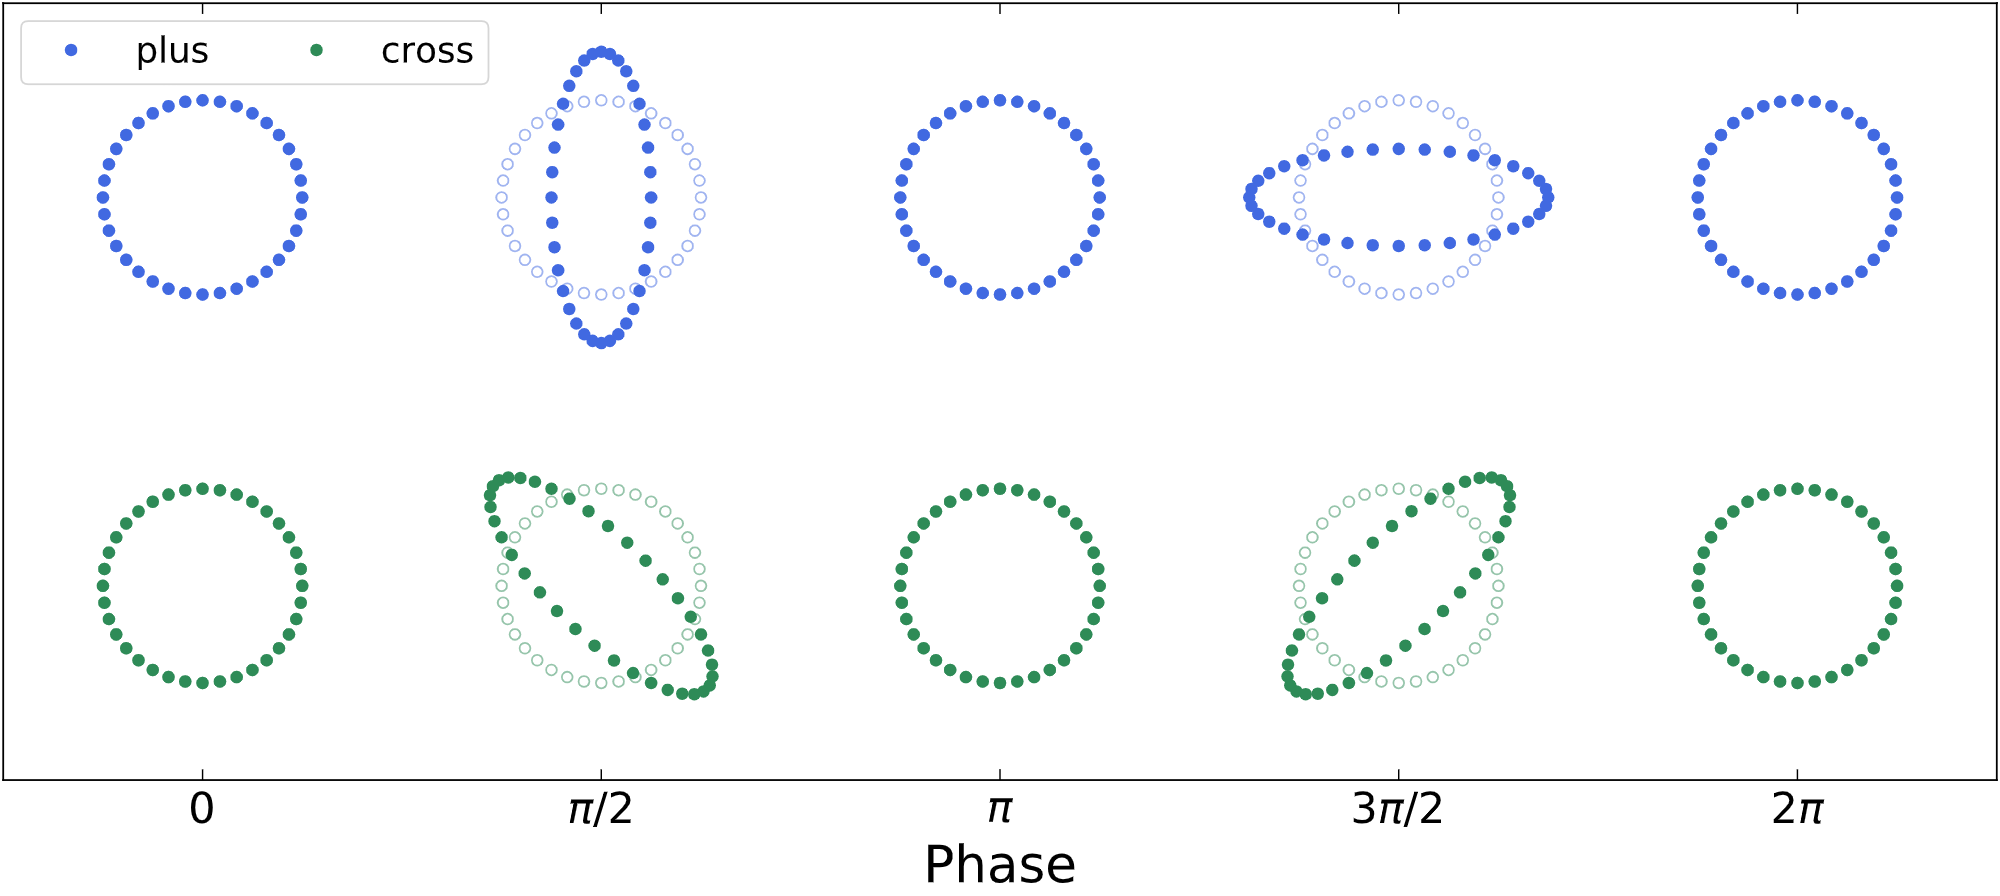
\includegraphics[width=\textwidth]{images/1_general_relativity/gravitational_radiation/polarisation.png}
   \caption{The effect of the two polarisations on a ring of test particles~\cite{gw_polarisation_plots}.}
   \label{1:fig:ring_of_particles}
\end{figure}
%
It can be seen that the effect of the $\times$ polarisation is the same as the $+$ polarisation but with a $45^{\circ}$ rotation.

\subsection{\label{1:sec:gw-emission}\Gwadj emission in linearised gravity}

We now return to Equation~\ref{1:eq:lorentz_gauge_efe} and reconsider the stress-energy tensor. The solution to the Einstein equations can be obtained using the Green's function~\cite{Dhurkunde:2024},
%
\begin{equation}
    \Bar{h}_{\mu\nu}(t, \vec{x}) = 4 \int d^3 x^{\prime} \frac{T_{\mu\nu}\left(t - |\vec{x} - \vec{x}^{\prime}|, \vec{x}^{\prime}\right)}{|\vec{x} - \vec{x}^{\prime}|},
    \label{1:eq:greens_functions}
\end{equation}
%
where the observer is at $\vec{x}$ and the source is at $\vec{x}^{\prime}$. The solution can be approximated using the quadrupole formula under two assumptions: the observer is far away $\left(|\vec{x} - \vec{x}^{\prime}| \approx |\vec{x}| = r\right)$ and the source velocity is small compared to the speed of light. 

We expand the stress-energy tensor using a Taylor expansion around the retarded time ($t - r$), and Equation~\ref{1:eq:greens_functions} simplifies to
%
\begin{equation}
    \Bar{h}_{\mu\nu}(t, \vec{x}) = \frac{4}{r} \int d^3 x^{\prime} T_{\mu\nu}\left(t - r, \vec{x}^{\prime}\right),
    \label{1:eq:quadrupole_simplification}
\end{equation}
%
to leading order. We can see that the \gws are dependent on the integral of the stress-energy tensor over a volume containing the source, evaluated at the retarded time.

Using the laws of conservation of total energy and momentum, $\partial^{\mu}T_{\mu\nu}=0$, we can see that the integral of the $T_{t\nu}$ and $T_{\nu t}$ components will be constant in time. We choose to ignore these components and focus only on observable signals in the spatial dimensions moving forward.

The right-hand side of Equation~\ref{1:eq:quadrupole_simplification} can be expressed as
%
\begin{equation}
    \frac{4}{r} \int d^3 x^{\prime} T_{ij} = \frac{2}{r}\frac{\partial^{2}}{\partial t^{2}} \int T_{00} x_{i} x_{j} d^{3} x^{\prime},
\end{equation}
%
where $T_{00} \approx \rho$, the Newtonian mass density. This expression is referred to as the \textit{mass quadrupole moment tensor} of the mass distribution
%
\begin{equation}
    M_{ij} := \int T_{00} x_{i} x_{j} d^{3} x^{\prime},
    \label{1:eq:quadrupole_moment_tensor}
\end{equation}
%
and when substituted into Equation~\ref{1:eq:quadrupole_simplification}, we obtain the \textit{quadrupole formula}
%
\begin{equation}
    h_{ij} = \frac{2}{r} \ddot{M}_{ij}(t-r),
    \label{1:eq:quadrupole_formula}
\end{equation}
%
where each dot over a tensor represents on derivative with respect to time.

The key properties of this equation are the dependence of gravitational radiation on the second time derivative of the quadrupole moment tensor, indicating that \gws are produced by rapid changes in the quadrupole moment tensor, such as the accelerations of masses and their directional changes during orbital cycles. Additionally, the \gwadj strain falls off inversely with distance $r$ from the source.

To extract the plus and cross polarisations of the metric perturbation we must now transform into the transverse-traceless gauge, this is done using the projection tensor~\cite{McIsaac_Thesis:2023}
%
\begin{equation}
    P^{i}_{j}(\hat{n}) = \delta^{i}_{j} - n^{i}n_{j}
\end{equation}
%
where
%
\begin{equation}
    P^{i}_{j}P^{j}_{k} = P^{i}_{k}
\end{equation}
%
and $\hat{n}$ is a normal vector such that $|\hat{n}| = 1$. Applying the projection vector to a three-dimensional vector will project it down into the two-dimensional plane orthogonal to $\hat{n}$. To get the components of $h_{ij}$ which are transverse to $\hat{n}$ we need to apply the projection tensor once for each index
%
\begin{equation}
    h^{T}_{kl} = P^{i}_{k}P^{j}_{l}h_{ij},
\end{equation}
%
and then to remove the trace of the tensor we use the Minkowski metric
%
\begin{equation}
    h^{T} = \eta^{ij}h^{T}_{ij} = P^{ij}h_{ij}.
\end{equation}
%
From this we can construct the tensor $\frac{1}{2}P_{kl}h^{T}$ which will have a trace of $h^{T}$ and will be transverse to $\hat{n}$ allowing us to subtract it from the transverse metric perturbation to get the metric perturbation in it's transverse-traceless form
%
\begin{equation}
    h^{TT}_{kl} = \Lambda^{,ij}_{kl} h_{ij} 
\end{equation}
%
where
%
\begin{equation}
    \Lambda^{,ij}_{kl} = \left(P^{i}_{k}P^{j}_{l} - \frac{1}{2}P_{kl}P^{ij}\right).
\end{equation}
%
Therefore, we can apply $\Lambda^{,ij}_{kl}$ to Equation~\ref{1:eq:quadrupole_formula} to get the transverse-traceless perturbation. For a gravitational wave travelling in the z-direction with $n^{i} = (0,0,1)$ (referred to as the "radiation" frame) we get plus and cross polarisations as functions of $\ddot{M}_{ij}$
%
\begin{equation}
    h_{+}^{TT} = \frac{G}{r}\left(\ddot{M}_{xx} - \ddot{M}_{yy}\right)
\end{equation}
%
\begin{equation}
    h_{\times}^{TT} = \frac{2G}{r}\left(\ddot{M}_{xy}\right).
\end{equation}

The total power radiated by a source is the \textit{luminosity flux}, and it must equal the energy carried by the \gws, due to the conservation of energy. We can obtain the luminosity flux by integrating the energy flux over a sphere with infinite radius from the source. The total energy loss rate is expressed as
%
\begin{equation}
    \frac{dE}{dt} = -\mathcal{L},
    \label{1:eq:de_dt}
\end{equation}
%
where $\mathcal{L}$ is the \gwadj luminosity flux. The luminosity flux at a large distance from the source is given by~\cite{Creighton_book:2009}
%
\begin{equation}
    L = \frac{1}{5} \left\langle \dddot{M}^{jk} \dddot{M}_{jk} \right\rangle,
    \label{1:eq:luminosity_flux}
\end{equation}
%
where the angular brackets represent averaging over all directions, and $\dddot{M}_{jk}$ refers to the third time derivative of the quadrupole moment. This shows that any source with a non-vanishing second derivative of its mass quadrupole moment will emit \gws.

Thus, through the quadrupole formula and \gwadj luminosity, we see that rapidly accelerating masses with a non-zero quadrupole moment are ideal sources of gravitational radiation.





















\section{\label{1:sec:gravitational-wave-detection}\Gwadj detection}

% Introduction to Gravitational Wave Detection
Having described the effect of \gws on a ring of particles, we now describe how these principles are applied to detect \gws on Earth. The first direct detection of \gws was achieved on the 14th September 2015~\cite{GW150914:2016}, made possible by ground-based \gwadj observatories. The current network of \gwadj detectors includes the Advanced LIGO (aLIGO) detectors located in Hanford and Livingston~\cite{aLIGO:2015}; Virgo in Italy~\cite{aVirgo:2015}; KAGRA in Japan~\cite{KAGRA:2021}; and GEO600 in Germany~\cite{GEO600:2002}. While this section will primarily focus on the design and operation of the aLIGO interferometers, the underlying detection principles are similar across all observatories. The configuration and performance of aLIGO are described comprehensively in~\cite{aLIGO:2015}.

\subsection{\label{1:sec:laser_interferometry}Laser interferometry}

% Basic Concept of Laser Interferometry
The physical effect of a passing \gw on a ring of particles (Figure~\ref{1:fig:ring_of_particles}) is described as a stretching and squeezing, changing the particles' proper distances depending on the polarisation of the \gw. The \gwadj observatories are Michelson interferometers, and we can visualise the L-shape of them as experiencing similar effects to the ring of particles. A basic diagram of the LIGO interferometer design can be seen in Figure~\ref{1:fig:ifo}.
%
\begin{figure}
    \centering
    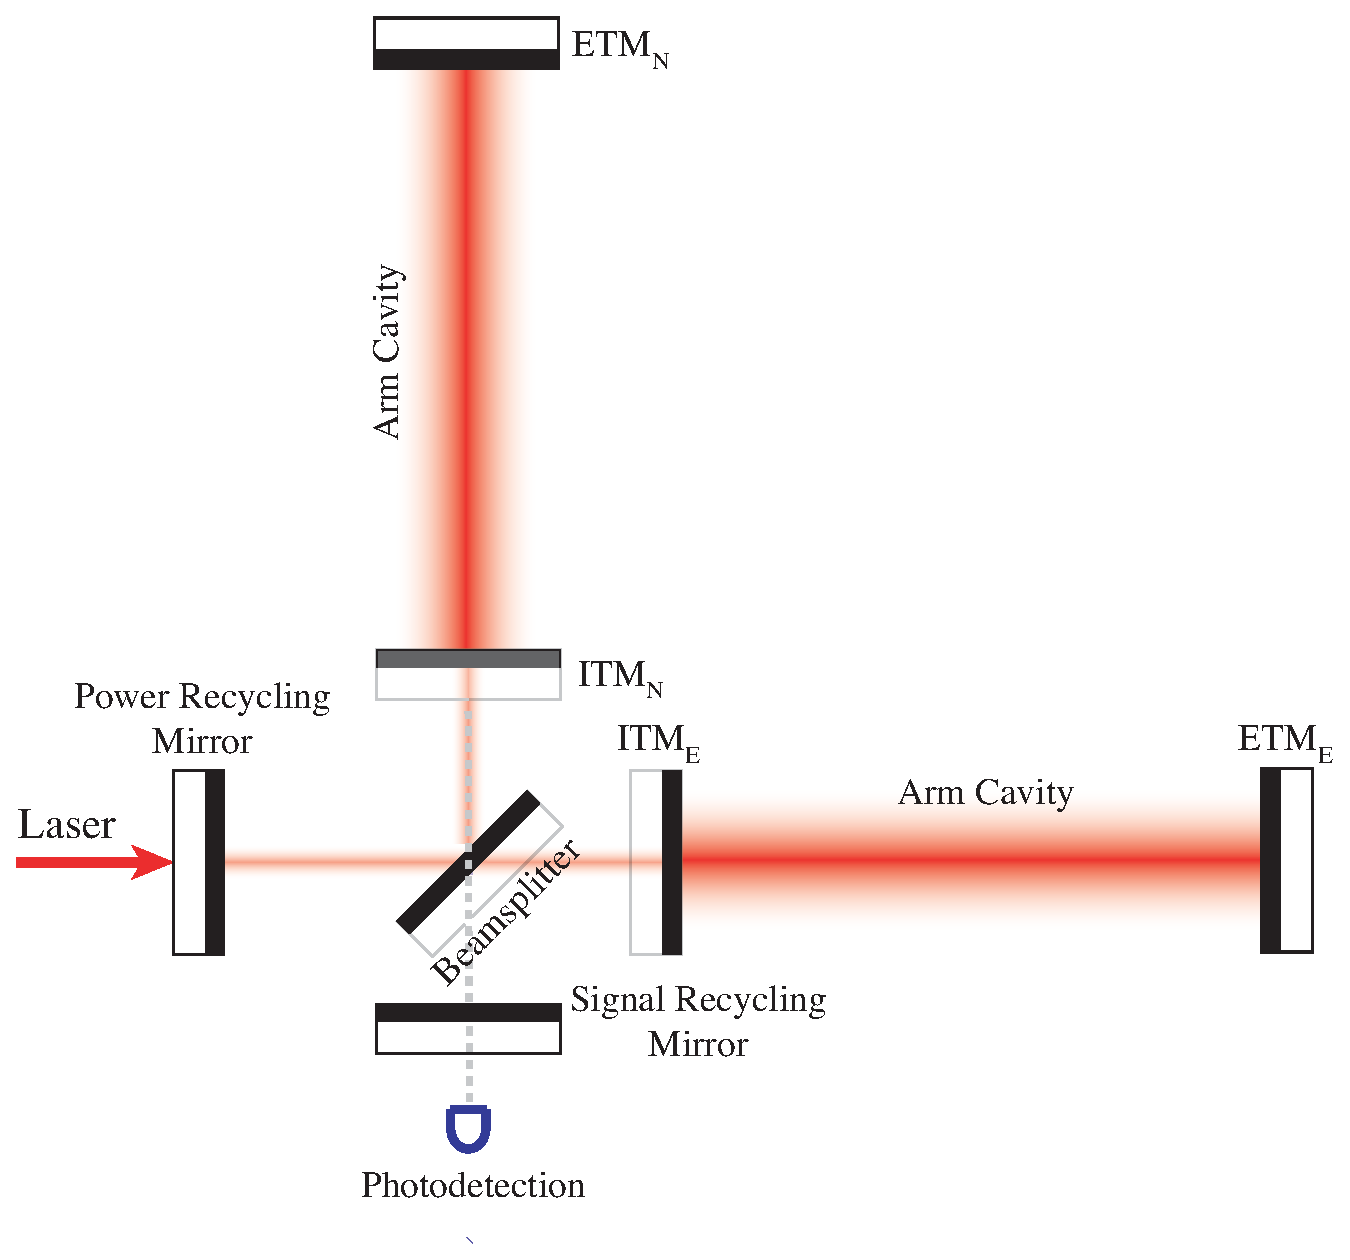
\includegraphics[width=0.9\linewidth]{images/1_general_relativity/gravitational_wave_detection/IFO.eps}
    \caption{An example Michelson laser interferometer detailing the main components of the advanced LIGO \gwadj observatory~\cite{aLIGO:2015}. Half the laser is reflected to the north arm cavity, physically defined by the input test mass (ITM$_{\text{N}}$) and the end test mass (ETM$_{\text{N}}$), and the other half is transmitted through to the east arm. Laser power builds up in the arm cavities through reflection between test masses before returning to the beam splitter, where there will be a total destructive interference of light when no \gwadj signal is present and therefore no signal will be measured at the photo-detector output. The power recycling mirror reflects laser light back into the detector arms to build up more power. The signal recycling mirror reflects light back into the arms with frequencies like those expected from \gwadj signals which resonates inside the cavity and increase the signal sensitive frequency power. Taken from~\cite{IFO_diagram:2008}.}
    \label{1:fig:ifo}
\end{figure}
%

Half the light from the laser incident on the beam splitter is transmitted to the end test mass in the $y$-direction (ETM$_{\text{N}}$) and half to the end test mass in the $x$-direction(ETM$_{\text{E}}$). The end test masses are mirrors which reflect the light back toward the beam splitter. When no \gw is present, the length of the $x$ and $y$ arm cavities are equal and the light returning to the beam splitter interferes destructively, meaning no light is detected by the photo-detector output of the detector.

% 
Using Equation~\ref{1:eq:proper_dist_two_particles}, where we are treating the detector arms like two particles placed at ($L, 0, 0$) for the end test mass of the $x$ arm and ($0, L, 0$) for the $y$-arm, we can calculate the change in arm length (proper distance) with respect to the beam splitter at the origin under the influence of a \gw propagating in the $z$-direction
%
\begin{equation}
    ds_{x} \approx \left(1 + \frac{1}{2}h_+\right)L,
\end{equation}
%
where $L$ is the length of the detector arm ($4 \, \text{km}$ for advanced LIGO) and in the $y$ arm
%
\begin{equation}
    ds_{y} \approx \left(1 - \frac{1}{2}h_+\right)L.
\end{equation}
%
The strain experienced by the $x$ and $y$ arms is directly related to both the magnitude of the $h_{+}$ \gwadj polarisation and the length of the detector arm. The arm in the $x$-direction will experience stretching, while the arm in the $y$-direction will experience squeezing.

% Calculating the Length Change in Interferometer Arms
The coupling of motion in both arms leads us to require the use of the differential change in arm length to calculate the \gwadj strain,
%
\begin{equation}
    h(t) = \frac{\delta L_1 - \delta L_2}{L},
    \label{1:eq:frac_length_diff_h_t}
\end{equation}
%
where $\delta L_{1}$ and $\delta L_{2}$ are the changes in the lengths of the arms.

We generalise $h(t)$ for any \gw of any polarisation. The strain induced in a single arm pointing in the $\mathbf{\vec{n}}$ direction, where $\mathbf{\vec{n}}$ is a unit normal vector, is
%
\begin{equation}
    \frac{\delta L}{L} = \frac{1}{2} h_{ij}n^{i}n^{j}
\end{equation}
%
and the difference in lengths for two interferometer arms is
%
\begin{equation}
    h(t) = \frac{1}{2} h_{ij}n_{1}^{i}n_{1}^{j} - \frac{1}{2} h_{ij}n_{2}^{i}n_{2}^{j},
\end{equation}
%
where crucially $h_{ij}$ is measured in the detector's reference frame. If our detector is located in the $x-y$ plane, the \gwadj signal is entirely polarised in the $h_{+}$ direction.

The \gw signal observed will depend on the orientation between source and detector. To transform between radiation frame and detector frame, we perform a set of rotations by angles ($\theta, \phi, \psi$) to adjust for the orientation and polarisation of the wave. Figure~\ref{1:eq:detector_frame_rotations} shows the required angles to describe effects on the \gwadj signal due to these transformations.
%
\begin{figure}
    \centering
    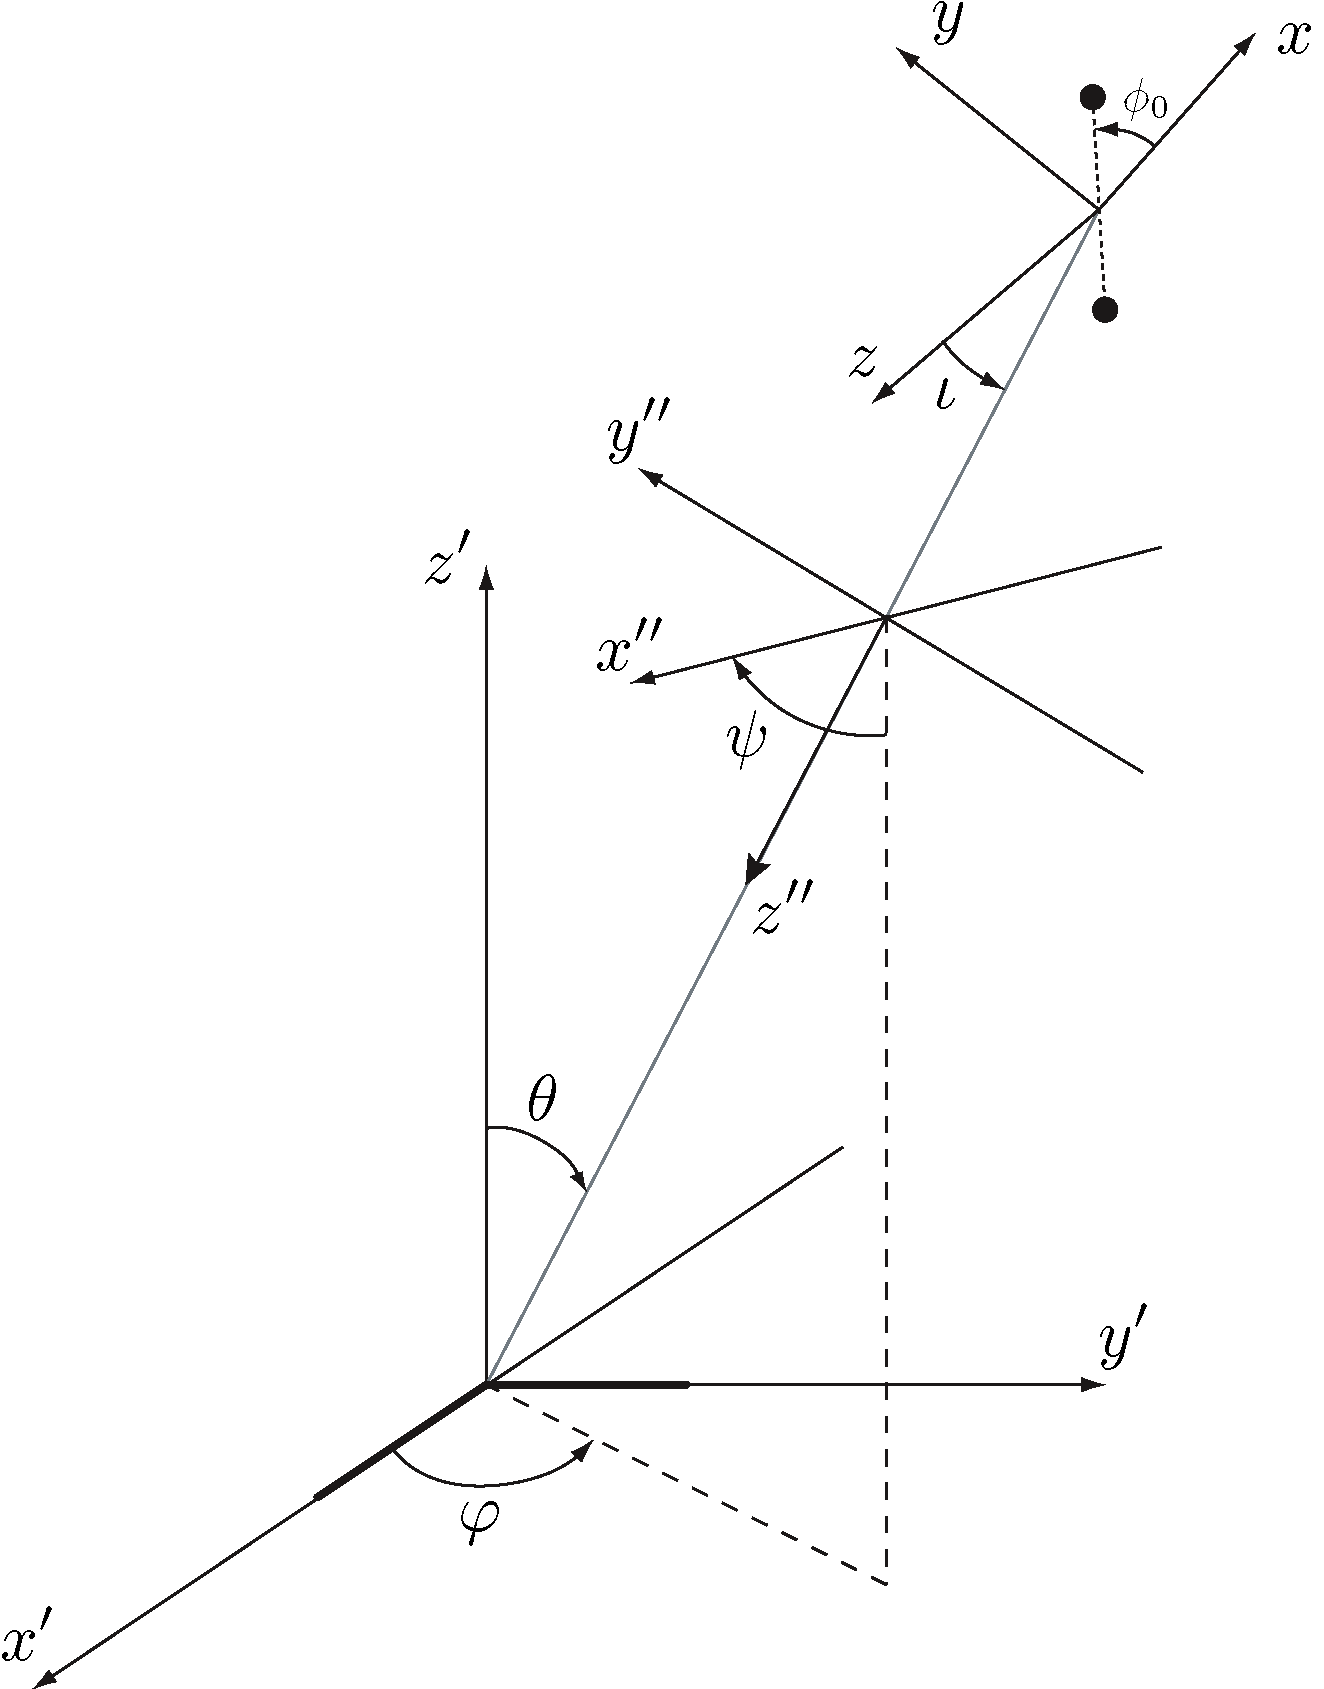
\includegraphics[width=0.75\linewidth]{images/1_general_relativity/gravitational_wave_detection/euler.png}
    \caption{The angles of rotation to describe a \gw from the source from (unprimed coordinates) to the detector frame (single primed coordinates) through the radiation frame (double primed coordinates). Taken from~\cite{Brown_Thesis:2004}.}
    \label{1:fig:source_to_detector_frame}
\end{figure}
%
Suppose we have a \gwadj signal in the radiation frame, to transform into the detector frame we must first define a rotation tensor
%
\begin{equation}
    R^{i}_{j} = 
    \begin{pmatrix}
        \cos\phi & -\sin\phi & 0 \\
        \sin\phi &  \cos\phi & 0 \\
        0        &  0        & 1
    \end{pmatrix}
    \begin{pmatrix}
        1 & 0 & 0 \\
        0 & \cos\theta & -\sin\theta \\
        0 & \sin\theta & \cos\theta \\
    \end{pmatrix}
    \begin{pmatrix}
        \cos\psi & -\sin\psi & 0 \\
        \sin\psi &  \cos\psi & 0 \\
        0        &  0        & 1
    \end{pmatrix},
    \label{1:eq:detector_frame_rotations}
\end{equation}
%
such that when transforming the spatial components of $h_{ij}$ using this tensor we can evaluate the detector strain as a function of the $+$ and $\times$ polarisations in the radiation frame and the three angles relating the radiation frame to the detector frame. A detector with arms aligned in the $x$ and $y$ directions will give
%
\begin{equation}
    h(t) = F_{+}(\Theta, \Phi, \Psi)h_{+}(t) + F_{\times}(\Theta, \Phi, \Psi)h_{\times}(t) ,
    \label{1:eq:h_t_linear_combination}
\end{equation}
%
where,
%
\begin{equation}
    F_{+}((\Theta, \Phi, \Psi)) = \frac{1}{2}(1 + \cos^{2}(\Theta))\cos2\Phi\cos2\Psi - \cos\Theta\sin2\Phi\sin2\Psi,
\end{equation}
%
\begin{equation}
    F_{\times}((\Theta, \Phi, \Psi)) = -\frac{1}{2}(1 + \cos^{2}(\Theta))\cos2\Phi\cos2\Psi - \cos\Theta\sin2\Phi\sin2\Psi
\end{equation}
%
which are the antenna responses of the detector to the $+$ and $\times$ polarisations respectively, which describe the sensitivity of the detector to \gws at different sky positions. 


\subsection{\label{1:sec:increase-det-sens}Increasing detector sensitivity}

% Relating Strain to Gravitational Wave Signal
With detector arm lengths on the order of ${\sim}10^{3} \, \text{m}$ and a laser wavelength of approximately $1 \, \mu\text{m}$, we are only able to measure a fractional change in the arm length on the order of $10^{-9} \, \text{m}$. However, our detectors are capable of measuring induced strain from passing \gws as small as $10^{-22}$. In this section, we discuss the detector improvements that enable these detections.

One technique used to effectively increase the arm length of the detectors is to allow the light to travel down the arms multiple times. The Fabry-Pérot cavities~\cite{aLIGO:2015} in the arms of the aLIGO detectors include an additional mirror on the input test mass (ITM), facing the end mirrors, which is highly reflective, allowing only a small fraction of light to transmit through. As a result, the light reflects multiple times between these two mirrors, increasing the optical path length to approximately $1000 \, \text{km}$. This also has the effect of building up laser power in the arms, sharpening the interference fringes to improve the ability to distinguish between noise and signal at the photo-detector~\cite{Meers:1988}.

Two additional components that increase detector sensitivity are: \textit{power recycling}, where a mirror at the laser input port redirects reflected light back into the interferometer, boosting the circulating power within the arms and enhancing the signal-to-noise ratio, enabling the detection of weaker \gwadj signals. The second improvement is the \textit{signal recycling mirror}, placed at the output port, which resonates with specific \gwadj frequencies, effectively increasing the detector's sensitivity to signals of interest. By tuning this mirror, the interferometer's sensitivity can be optimized for certain frequency bands. These improvements together allow the detector to reach sensitivities capable of observing strain on the order of $10^{-22}$ for short-duration signals up to a few seconds long.

\section{\label{1:sec:modelling_CBC}Modelling compact binary coalescences}

The primary sources of \gws seen by Earth-based \gwadj detectors are those from \cbcs. \Cbcs (CBC) are the inspiral and merger of two compact objects (black holes or neutron stars). The binary system will emit \gws and slowly dissipate the orbital energy of the system. The system is locked in the cycle of a decreasing orbit leading to greater acceleration, increasing the rate at which energy is being dissipated and the orbital radius decreases. The orbit will decay until an eventual merger between the two objects. We have observed three distinct CBC systems: binary black holes~\cite{GW150914:2016} (BBH), binary neutron stars~\cite{GW170817:2017} (BNS) and neutron star — black hole binaries~\cite{nsbh:2021}. 

In this section, we describe the \gws emitted by a CBC and the physical effects these would have on \gwadj detectors. First, we need to describe the intrinsic parameters of the \gwadj signal being created and the extrinsic, observational parameters which affect the signal based on how it is being observed. Next, we derive a gravitational waveform with a very simple binary system of two point-like masses using the Newtonian formalism.

\subsection{\label{1:sec:CBC-parameters}Waveform parameters}

\subsubsection{Intrinsic parameters}
The intrinsic parameters are those which have physical effects on the system and alter how the \gwadj signal is created,
\begin{itemize}
   \item Primary and secondary component masses, $m_{1}$ and $m_{2}$
   \item Primary and secondary three-dimensional spin vectors, $\vec{s_{1}}$ and $\vec{s_{2}}$
\end{itemize}
Here, the subscript $_1$ refers to the more massive object in the binary system, and $_2$ to the less massive one.

\subsubsection{Extrinsic parameters}
The extrinsic parameters affect how the \gwadj signal is observed,
\begin{itemize}
   \item Right ascension of the source location, $\alpha$ 
   \item Declination of the source location, $\delta$
   \item Luminosity distance to the source, $r$, 
   \item Inclination angle between the line of sight and the orbital angular momentum of the binary, $\iota$
   \item Polarisation angle of the \gw, $\psi$
   \item Time of coalescence, $t_{c}$
   \item Coalescence phase, $\phi_{c}$ 
\end{itemize}

There are additional parameters that describe other physical effects such as: tidal deformations, eccentricity, the neutron star equation of state, or potential deviations from \GR. In this work, we will ignore these additional effects and focus on the $15$ parameters listed above.

\subsection{\label{1:sec:keplerian_derivation}Simple CBC inspiral}

We can derive $h_{+}$ and $h_{\times}$ for a binary system modelled as a decaying quasi-circular orbit of two point masses around a shared centre of mass. These two point masses are in the `inspiral' regime, where they are radiating \gws, travelling with speeds much less than $c$ and, are not close to merging. We choose a frame of reference where the plane of the binary is in the $x$-$y$ direction and the binary is situated at a distance $r$ from the observer.

Assuming a circular orbit, we obtain the orbital velocity in Kepler's laws of planetary motion by equating the Newtonian gravitational force and the orbital centripetal force
%
\begin{align}
    \frac{m_{1} m_{2}}{a^{2}} = \frac{\mu v^{2}}{a}, \\
    v = \sqrt{\frac{m_{1} + m_{2}}{a}},
\end{align}
%
where $m_{1}$ and $m_{2}$ are the masses of the objects, $\mu$ is the reduced mass of the system ($\mu = \frac{m_1m_2}{(m_1+m_2)}$) and $a$ is the distance between the two objects.
%
Using $\omega = v/a$, we can obtain the orbital frequency
%
\begin{equation}
    \omega_{orbit} = \sqrt{\frac{m_{1} + m_{2}}{a^{3}}},
    \label{1:eq:omega_orbit}
\end{equation}
%
and relate it to the rate of change in the orbital phase
%
\begin{equation}
    \omega_{orbit} = \frac{d \Phi_{orbit}}{dt}.
\end{equation}
%
Using the quadrupole formula (Equation~\ref{1:eq:quadrupole_formula}), we can derive the metric perturbations caused by this system
%
\begin{equation}
    h_{\mu\nu} = \frac{4}{r} \mu a^{2} \omega^{2}_{orbit}
    \begin{pmatrix}
      0 & 0 & 0 & 0 \\
      0 & -\cos\left(2\omega_{orbit}t\right) & -\sin\left(2\omega_{orbit}t\right) & 0 \\
      0 & -\sin\left(2\omega_{orbit}t\right) & \cos\left(2\omega_{orbit}t\right) & 0 \\
      0 & 0 & 0 & 0
   \end{pmatrix}.
\end{equation}
%
The line of sight between the binary system and the observer is defined by the inclination angle, $\iota$, and when projecting the \gwadj emission in the line of sight we get the waveform polarisations,
%
\begin{equation}
    h_{+}(t) = \frac{4}{r} M\eta v^{2} \left(\frac{1 + \cos^{2}\iota}{2}\right)\cos\left(2\omega_{orbit}t+2\Phi_{c}\right),
\end{equation}
%
\begin{equation}
    h_{\times}(t) = \frac{4}{r} M\eta v^{2} \left(\frac{\cos\iota}{2}\right)\sin\left(2\omega_{orbit}t+2\Phi_{c}\right),
\end{equation}
%
where $M = m_1 + m_2$ is the total mass of the system, $\eta = \frac{m_{1}m_{2}}{(m_{1} + m_{2})^{2}}$ is the symmetric mass ratio and $\Phi_{c}$ is the coalescence phase of the system. A key observation from these equations is that the frequency of the \gws is twice that of the binary orbital frequency.

We have an embedded assumption that the separation distance of the two objects will remain constant. We know that the radiation of \gws will decrease the orbit of the binary system, and so by solving equations~\ref{1:eq:de_dt} and~\ref{1:eq:luminosity_flux}, we can find the power radiated by the binary system. The energy loss will increase the binary orbital frequency, from this we can calculate the change in phase and amplitude as a function of time.

In the two point source example we relate the orbital velocity, $\omega_{orbit}$ to the particle separation, $a$, using Equation~\ref{1:eq:omega_orbit} and then when introducing the \textit{chirp mass}, $\mathcal{M}$, of the binary system
%
\begin{equation}
    \mathcal{M} = \frac{(m_{1}m_{2})^{\frac{3}{5}}}{(m_{1} + m_{2})^\frac{1}{5}},
\end{equation}
%
and solving equations~\ref{1:eq:de_dt} and~\ref{1:eq:luminosity_flux} we are able to determine the power radiated by this system as
%
\begin{equation}
    \frac{dE}{dt} = -\frac{32}{5}(\mathcal{M}\omega_{orbit})^\frac{10}{3}.
    \label{1:eq:cbc_eg_de_dt}
\end{equation}
%
The total energy of the system can be expressed as
%
\begin{align}
    E &= -\frac{m_{1}m_{2}}{2a}, \\
      &=-\frac{1}{2}(\mathcal{M}^{5} \omega^{2}_{orbit})^\frac{1}{8},
      \label{1:eq:total_energy_cbc}
\end{align}
%
and when substituted into Equation~\ref{1:eq:cbc_eg_de_dt} and solving we obtain the orbital frequency as a function of time
%
\begin{align}
    \omega_{orbit}(t) &= \left(-\frac{256}{5}\mathcal{M}^{\frac{5}{3}}(t - t_{0})\right)^{-\frac{3}{8}}, \\
                      &= \frac{1}{8}\left(\frac{\tau}{5}\right)^{-\frac{3}{8}}\mathcal{M}^{-\frac{5}{8}},
    \label{1:eq:omega_orbit_f_of_tau}
\end{align}
%
where $t_{0}$ is the fiducial starting time for integration which is used to map the time to define a new time variable $\tau = t_{c} - t$.


We can integrate Equation~\ref{1:eq:omega_orbit_f_of_tau} over time to find the orbital phase of the \gwadj signal,
%
\begin{align}
    \Phi(\tau) &= \int^{t}_{t+{0}} \omega_{orbit} dt, \\ 
    &= -2\left(\frac{5G\mathcal{M}}{c^{3}}\right)^{-\frac{5}{8}} \tau^{\frac{5}{8}} + 2\Phi_{c},
\end{align}
%
where $\Phi_{c}$ is the coalescence phase.

Finally, combining the previous equations, we have derived
%
\begin{equation}
    h_{+}(\tau) = \frac{1}{r}\left(\frac{G\mathcal{M}}{c^{2}}\right)^{\frac{5}{4}}\left(\frac{5}{c\tau}\right)^{\frac{1}{4}}\left(\frac{1+\cos^{2}\iota}{2}\right)\cos\Phi(\tau),
\end{equation}
%
\begin{equation}
    h_{\times}(\tau) = \frac{1}{r}\left(\frac{G\mathcal{M}}{c^{2}}\right)^{\frac{5}{4}}\left(\frac{5}{c\tau}\right)^{\frac{1}{4}}\cos\iota\sin\Phi(\tau),
\end{equation}
%
the \gwadj polarisations for a metric perturbation originating from our simple two-point particle binary system. From these equations, it's easy to show that both the amplitude and frequency of the system will increase rapidly and ``chirp'' as it approaches coalescence. Also clear to see is that these \gwadj signals are dependent only on the chirp mass of the system.

\subsection{\label{1:sec:fourier_transform_chirp}Fourier transform of the chirp signal}

In \gwadj analysis, the Fourier transform of a chirp signal is crucial for understanding its frequency domain characteristics. We consider a gravitational waveform given by
%
\begin{equation}
    h(t) = A(t) \cos \Phi(t),
\end{equation}
%
where \( A(t) \) represents the amplitude, and \( \Phi(t) \) is the phase of the signal. To simplify our analysis, we use the \textit{stationary phase approximation}, applicable when the amplitude \( A(t) \) varies slowly compared to the phase \( \Phi(t) \). Under this approximation, the Fourier transform of \( h(t) \) is given by
%
\begin{equation}
    \Tilde{h}(f) \simeq \frac{1}{2} A\left(t(f)\right) \left(\frac{dt(f)}{df}\right)^{\frac{1}{2}} {\rm e}^{i \left(2\pi f t(f) - \Phi(f) - \frac{\pi}{4}\right)},
\end{equation}
%
where \( t(f) \) and \( \Phi(f) \) are the time and phase at frequency \( f \). For a chirp signal, these quantities can be expressed as
%
\begin{equation}
    t(f) = t_c - \frac{5}{8\pi}\left(8\pi f\right)^{-\frac{8}{3}} \mathcal{M}^{-\frac{5}{3}},
\end{equation}
%
\begin{equation}
    \Phi(f) = \Phi_c - 2\left(8\pi \mathcal{M} f\right)^{-\frac{5}{3}},
\end{equation}
%
where \( t_c \) is the coalescence time, \( \mathcal{M} \) is the chirp mass, and \( \Phi_c \) is the phase at coalescence.

The Fourier transform of the chirp signal, considering the Newtonian approximation, can be expressed in the form of
%
\begin{equation}
    \Tilde{h}(f) = \sqrt{\frac{5}{24}} \frac{G^2 \mathcal{M}^2}{c^5 d_L} \left(\frac{\pi G \mathcal{M} f}{c^3}\right)^{-\frac{7}{6}} \left(\frac{1 + \cos^2 \iota}{2}\right) {\rm e}^{i \Phi(f; t_c)},
\end{equation}
%
where the phase term \( \Phi(f; t_c) \) is defined by
%
\begin{equation}
    \Phi(f; t_c) = \frac{\pi}{4} - \frac{3}{128} \left(\frac{\pi G \mathcal{M} f}{c^3}\right)^{-\frac{5}{3}} - 2\pi f t_c + \Phi_c.
\end{equation}
%
Here, \( d_L \) denotes the luminosity distance to the source, and \( \iota \) is the inclination angle of the orbital plane with respect to the line of sight.

\subsection{\label{1:sec:post_newtonian_treatment}Post-Newtonian approximation}

Our Newtonian model of the \gwadj signal from a CBC source has been derived with simplifications. However, the real signals detected by \gwadj detectors are far more complex, requiring corrections to account for the effects of \GR. The post-Newtonian (PN) expansion technique improves the accuracy of gravitational waveforms by introducing relativistic corrections to the waveform, accounting for deviations from Newtonian gravity due to \GR~\cite{2PN_1:1996, 2PN_2:1996, 2PN_3:1995}.

The PN expansion can be performed by expanding in powers of \( v/c \), where \( v \) is the velocity of the orbiting bodies, to obtain the corrections to the waveform which can then be summed to get waveforms up to the required PN order. For a CBC, the waveform could be written as
%
\begin{equation}
    h(t) = h_{\text{Newtonian}}(t) + h_{\text{1PN}}(t) + h_{\text{1.5PN}}(t) + h_{\text{2PN}}(t) + \cdots,
\end{equation}
%
where \( h_{\text{Newtonian}}(t) \) is the leading-order Newtonian term, and the following terms represent higher and higher PN order corrections~\cite{PN_models:2009}.

\subsection{\label{1:sec:full_waveform}Full waveform}

The post-Newtonian (PN) formalism is accurate during the inspiral phase of the waveform when the two objects are still distant from each other, and formalism does not cover the entire evolution of the system. The system continues to emit \gws throughout the merger and post-merger phases, including the ringdown phase, where the newly formed object settles into its final shape. The \gwadj emission peaks during the merger, making it crucial for detecting \gws. The ringdown phase is particularly valuable for testing General Relativity (GR)~\cite{GW150914_TGR:2016, GW170817_TGR:2019, O3_TGR:2021}.

Generating full waveforms requires solving the Einstein field equations using numerical relativity (NR), a process that can take weeks. To efficiently model the entire evolution of the waveform---comprising the inspiral, merger, and ringdown (IMR) phases (see Figure~\ref{1:fig:IMR})---waveform families use a combination of NR waveforms and analytical or semi-analytical approximations. This approach balances accuracy with computational efficiency. The following subsections briefly describe these waveform models.

\begin{figure}
    \centering
    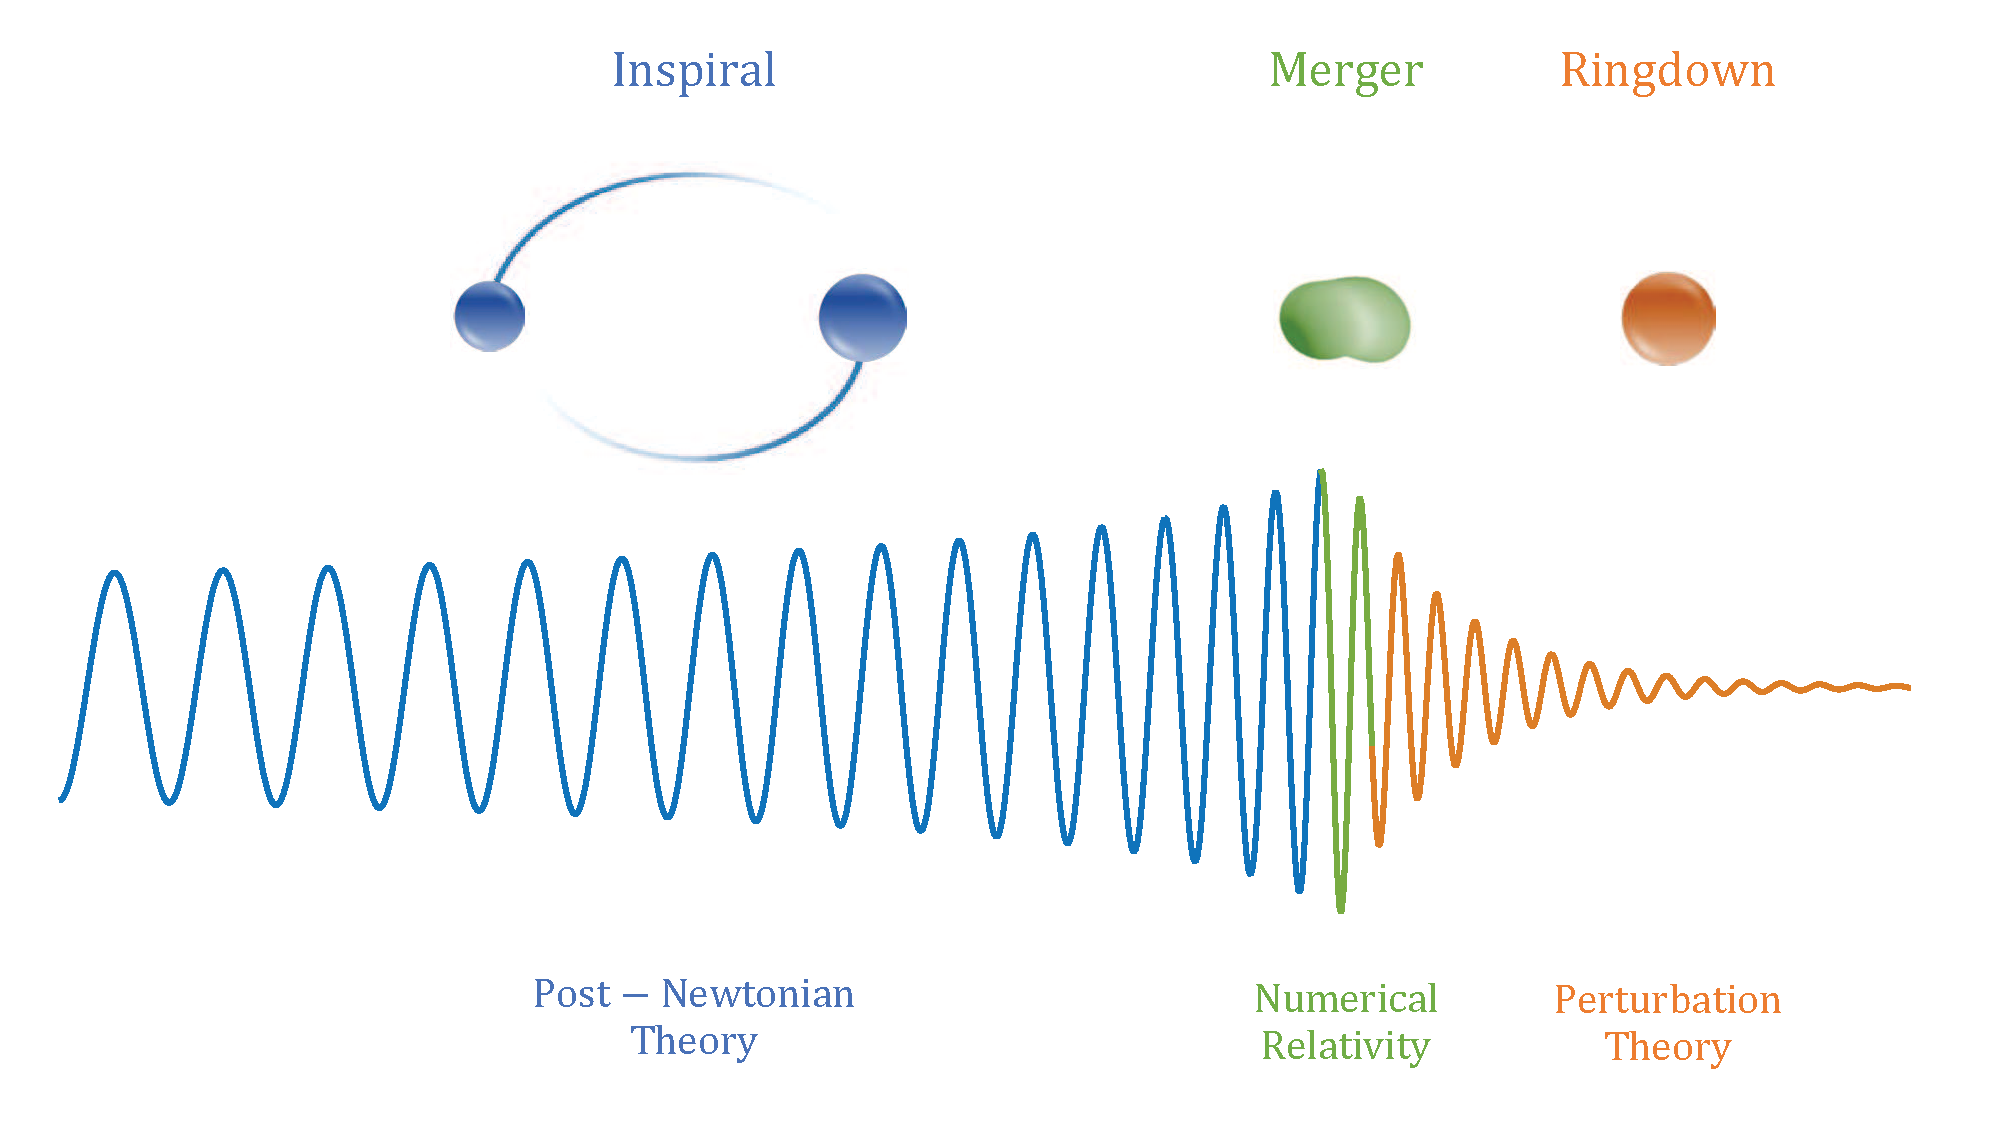
\includegraphics[width=0.75\linewidth]{images/1_general_relativity/modelling_cbc/IMR.pdf}
    \caption{The evolution of a compact binary merger is illustrated through three distinct phases. The inspiral phase involves the two compact objects orbiting each other, with the orbit decaying as they emit \gws. This phase is modelled using post-Newtonian theory. The merger phase occurs when the orbital radius decreases sufficiently for the objects to merge into a new compact object, modelled using numerical relativity. The ringdown phase represents the newly formed object's vibration as it settles into its final shape, modelled using perturbation theory. This image is adapted from~\cite{IMR_plot:2016}.}
    \label{1:fig:IMR}
\end{figure}

\subsubsection{Effective-One-Body (EOB)}

The Effective-One-Body (EOB) model~\cite{EOB_1:1998} simplifies the binary system by transforming it into an equivalent single test particle moving in an external gravitational field, described by a Hamiltonian~\cite{EOB_1:1998, EOB_2:2000, EOB_3:2000, EOB_4:2001}. This Hamiltonian includes both leading-order Newtonian terms and higher-order post-Newtonian corrections~\cite{EOB_5:2008}.

EOB models tuned to numerical relativity (NR) data are known as ``EOBNR'' models~\cite{EOB_6:2007}. Some of these models, such as \texttt{SEOBNRv5}~\cite{SEOBNRv5:2023tna}, also incorporate the effects of anti-aligned spins. Further enhancements allow for precession effects and higher-order modes of \gwadj emission, as seen in the state-of-the-art model \texttt{SEOBNRv5\_PHM}~\cite{SEOBNRv5_PHM-Buades:2023ehm}, which represents the most advanced EOB waveform model as of the drafting of this thesis.

\subsubsection{Phenomenological models}

Phenomenological models, often abbreviated as `Phenom', use a phenomenological ansatz calibrated with NR simulations to produce full waveforms. These models are fully analytical and can generate both Fourier domain and time domain waveforms~\cite{IMR_1:2007, IMR_2:2020}. The ability to create waveforms directly in the Fourier domain is highly desirable for analyses that require generating millions of waveforms, such as offline searches or parameter estimation.

Phenom models that cover the inspiral, merger, and ringdown phases are prefixed with \texttt{IMRPhenom}~\cite{IMRPhenomD:2009}. The state-of-the-art model of this family is \texttt{IMRPhenomXPHM}~\cite{IMRPhenomXPHM:2020}, which can accurately model anti-aligned spins, precessing binaries (\texttt{P}), higher-order modes (\texttt{HM}), and extreme mass ratios (\texttt{X}).

\subsubsection{Surrogate models}

Surrogate models create waveforms by interpolating from NR simulations~\cite{Surr_1:2019, Surr_2:2022}. These models, such as \texttt{NRSur7dq4}~\cite{NRSur7dq4:2019}, provide greater accuracy than other model families but are limited by the parameter regions covered by the NR simulations used for interpolation. The current leading surrogate model, \texttt{NRSur7dq4}, is valid up to a mass ratio of four.
